\documentclass{article}
\usepackage[utf8]{inputenc}
\usepackage[margin=1in]{geometry}
\usepackage{amsmath}
\usepackage{amsfonts}
\usepackage{amssymb}
\usepackage{graphicx}
\usepackage{booktabs}
\usepackage{array}
\usepackage{multirow}
\usepackage{float}
\usepackage{caption}
\usepackage{subcaption}
\usepackage{xcolor}
\usepackage{url}
\usepackage{longtable}

\title{\textbf{Decision Tree Analysis}}
\author{Nafis Nahian \\ CSE 318 - Artificial Intelligence Lab}
\date{\today}

\begin{document}

\maketitle

\section{Introduction}

Decision trees are fundamental machine learning algorithms that create predictive models through recursive binary splits. The choice of splitting criterion significantly impacts tree performance, accuracy, and generalization capability. This study compares three splitting criteria:

\begin{itemize}
    \item \textbf{Information Gain (IG)}: Measures reduction in entropy after splitting
    \item \textbf{Information Gain Ratio (IGR)}: Normalizes IG by split information to reduce bias toward multi-valued attributes
    \item \textbf{Normalized Weighted Information Gain (NWIG)}: A weighted variant considering attribute importance
\end{itemize}

\section{Experimental Setup}

\subsection{Datasets}
Two benchmark datasets were used:
\begin{itemize}
    \item \textbf{Adult Dataset}: 32,562 records with binary classification (income greater than or less than 50K)
    \item \textbf{Iris Dataset}: 150 records with 3-class classification (iris species)
\end{itemize}

\subsection{Methodology}
\begin{itemize}
    \item 20 independent runs with 80\%-20\% train-test split
    \item Maximum tree depths: 2, 3, and 4
    \item Metrics: Accuracy, training time, testing time, and total nodes
\end{itemize}

\section{Results}

\subsection{Accuracy Analysis}

\subsubsection{Adult Dataset}
Table \ref{tab:adult_accuracy} presents the accuracy results for the Adult dataset across different criteria and depths.

\begin{table}[H]
\centering
\caption{Adult Dataset Accuracy Results (\%)}
\label{tab:adult_accuracy}
\begin{tabular}{@{}lccc@{}}
\toprule
\textbf{Criteria} & \textbf{Depth 2} & \textbf{Depth 3} & \textbf{Depth 4} \\
\midrule
IG & 81.98 & 82.37 & 82.05 \\
IGR & \textbf{83.36} & \textbf{83.35} & \textbf{86.02} \\
NWIG & 81.97 & 82.27 & 81.76 \\
\bottomrule
\end{tabular}
\end{table}

\subsubsection{Iris Dataset}
Table \ref{tab:iris_accuracy} shows the accuracy results for the Iris dataset.

\begin{table}[H]
\centering
\caption{Iris Dataset Accuracy Results (\%)}
\label{tab:iris_accuracy}
\begin{tabular}{@{}lccc@{}}
\toprule
\textbf{Criteria} & \textbf{Depth 2} & \textbf{Depth 3} & \textbf{Depth 4} \\
\midrule
IG & 92.00 & 91.67 & 92.67 \\
IGR & 93.67 & \textbf{95.00} & 94.67 \\
NWIG & 92.00 & 91.67 & 92.67 \\
\bottomrule
\end{tabular}
\end{table}

\subsection{Tree Complexity Analysis}

\subsubsection{Node Count Comparison}
Table \ref{tab:nodes_comparison} compares the average total nodes across criteria and depths.

\begin{table}[H]
\centering
\caption{Average Total Nodes Comparison}
\label{tab:nodes_comparison}
\begin{tabular}{@{}lcccccc@{}}
\toprule
\multirow{2}{*}{\textbf{Criteria}} & \multicolumn{3}{c}{\textbf{Adult Dataset}} & \multicolumn{3}{c}{\textbf{Iris Dataset}} \\
\cmidrule(lr){2-4} \cmidrule(lr){5-7}
& \textbf{D=2} & \textbf{D=3} & \textbf{D=4} & \textbf{D=2} & \textbf{D=3} & \textbf{D=4} \\
\midrule
IG & 92 & 1,103 & 4,899 & 20 & 31 & 35 \\
IGR & \textbf{240} & \textbf{290} & \textbf{525} & 22 & \textbf{25} & \textbf{27} \\
NWIG & 127 & 1,307 & 5,278 & 20 & 30 & 34 \\
\bottomrule
\end{tabular}
\end{table}

\subsection{Computational Performance}
Table \ref{tab:timing} summarizes the training and testing times for the Adult dataset.

\begin{longtable}{lccc}
\hline
\multirow{2}{*}{\textbf{Criteria}} & \multicolumn{3}{c}{\textbf{Training Time (s)}} \\ \cline{2-4} 
 & \textbf{Depth=2} & \textbf{Depth=3} & \textbf{Depth=4} \\ \hline
\endhead
%
IG & 0.64 & 3.41 & 40.94 \\
IGR & \textbf{1.15} & \textbf{1.36} & \textbf{2.04} \\
NWIG & 0.6 & 2.5 & 32.53 \\ \hline
\caption{Adult Dataset Computational Performance}
\label{tab:timing}\\
\end{longtable}

\section{Visualizations}

\subsection{Accuracy vs Depth Analysis}

Figure \ref{fig:accuracy_bars} shows the accuracy comparison across different depths and criteria for both datasets.

\begin{figure}[H]
\centering
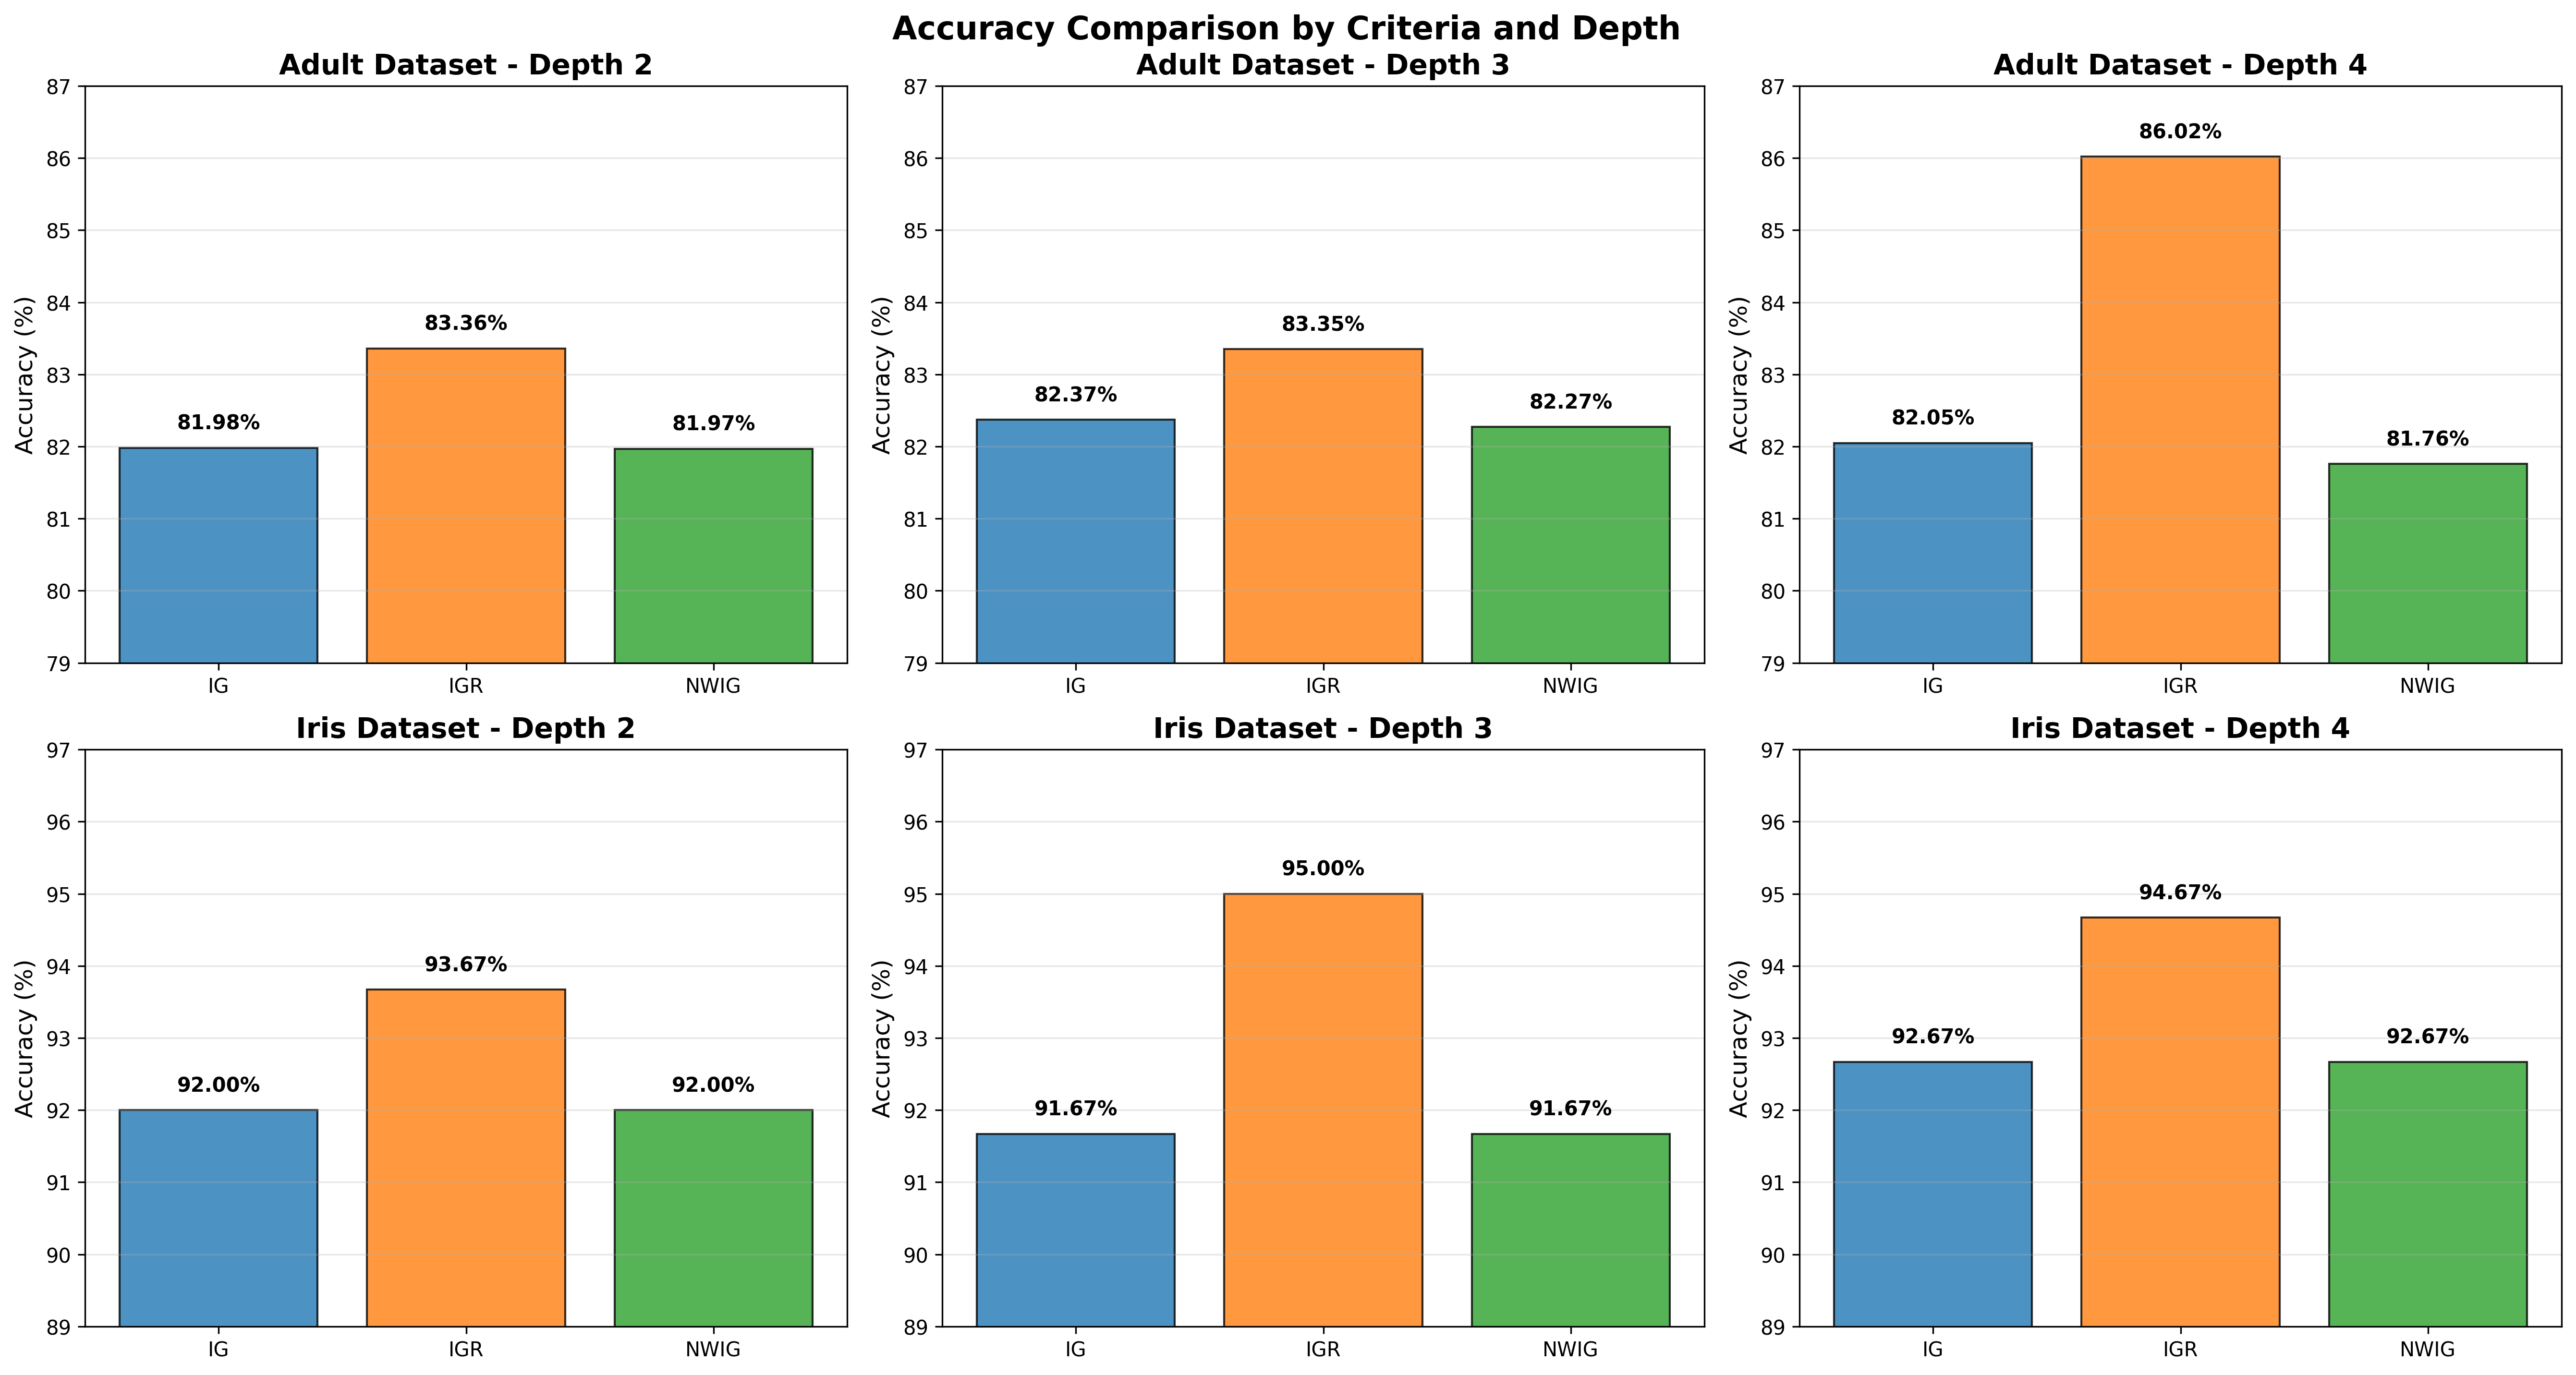
\includegraphics[width=0.95\textwidth]{accuracy_bar_plots_by_depth.png}
\caption{Accuracy Comparison by Criteria and Depth for Both Datasets}
\label{fig:accuracy_bars}
\end{figure}

Figure \ref{fig:accuracy_combined} provides a direct comparison between datasets for each depth level.

\begin{figure}[H]
\centering
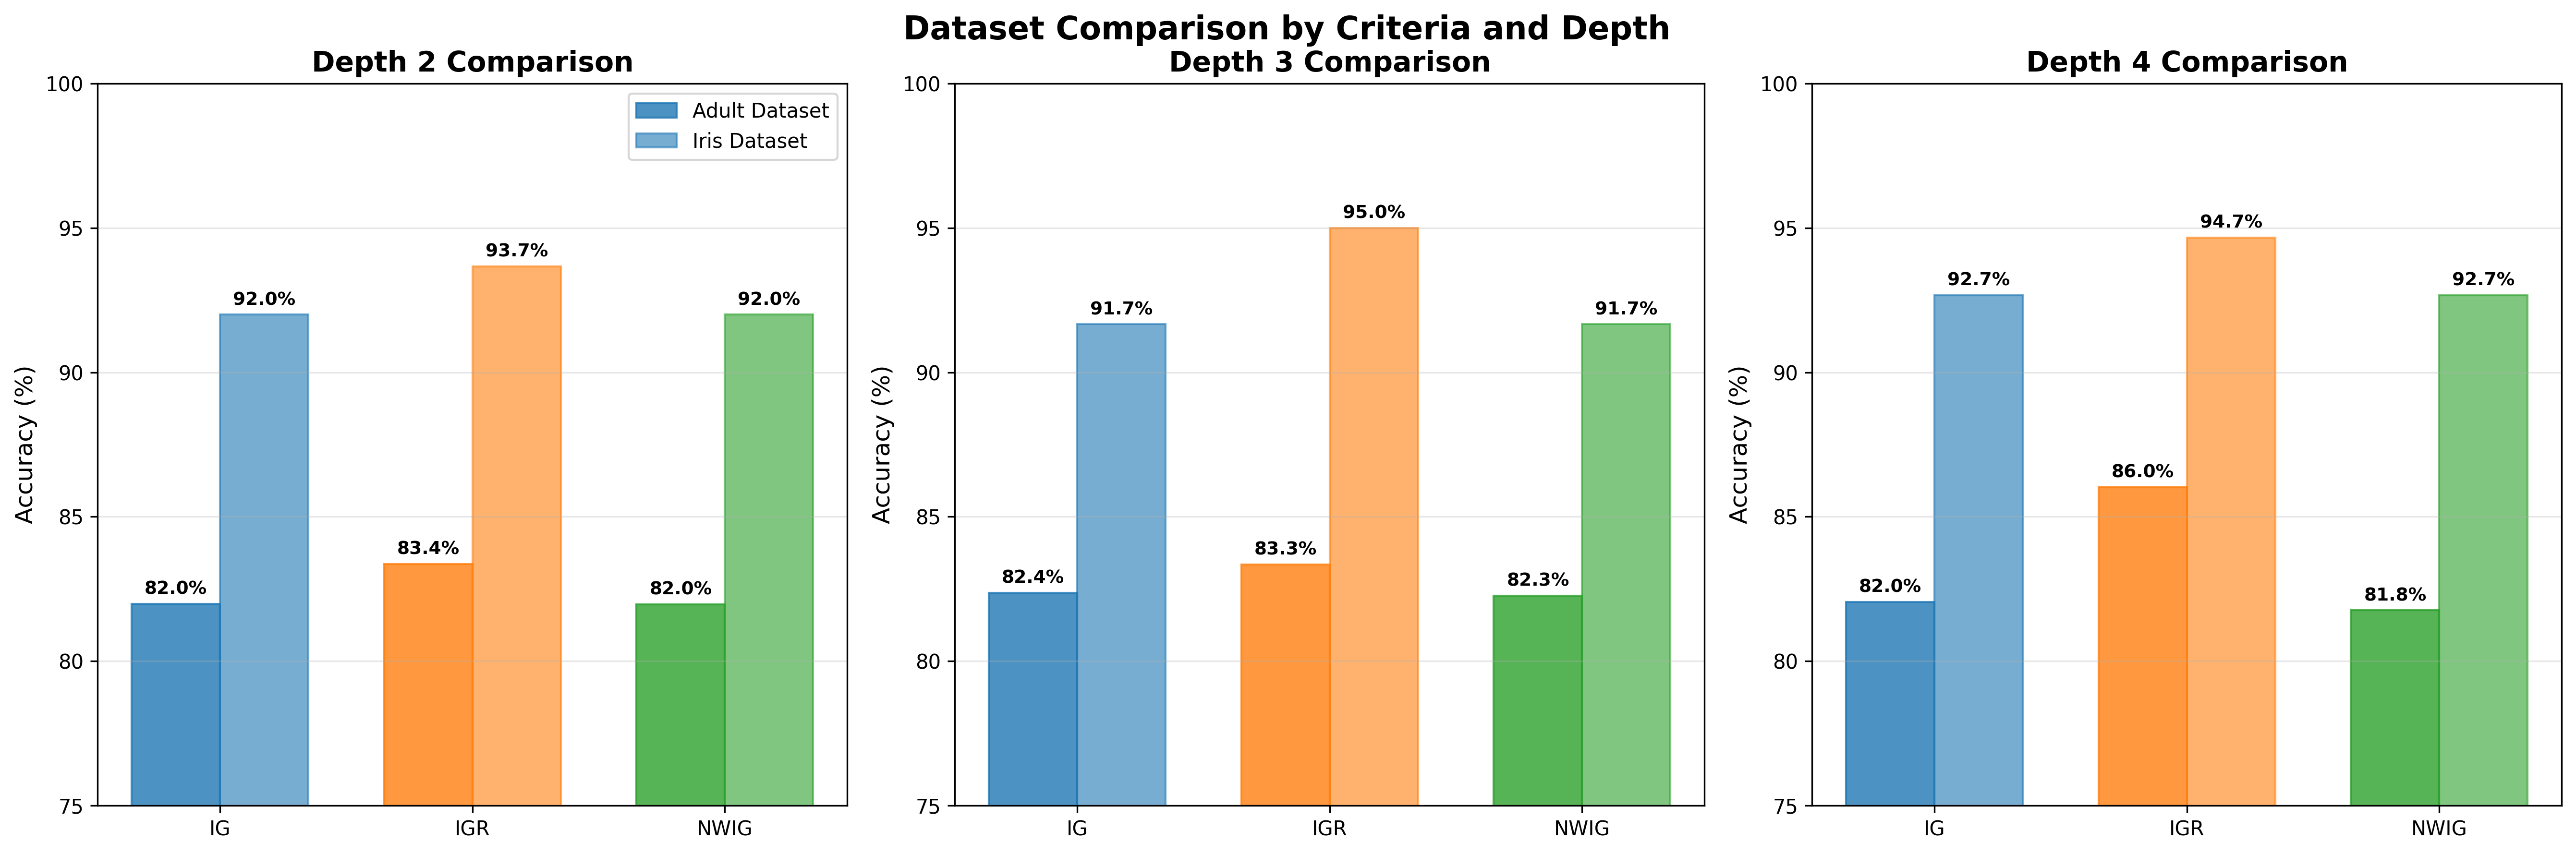
\includegraphics[width=0.95\textwidth]{combined_bar_comparison_by_depth.png}
\caption{Dataset Comparison by Criteria and Depth}
\label{fig:accuracy_combined}
\end{figure}

\subsection{Tree Complexity Analysis}

Figure \ref{fig:nodes_bars} illustrates the relationship between tree depth and complexity measured by node count.

\begin{figure}[H]
\centering
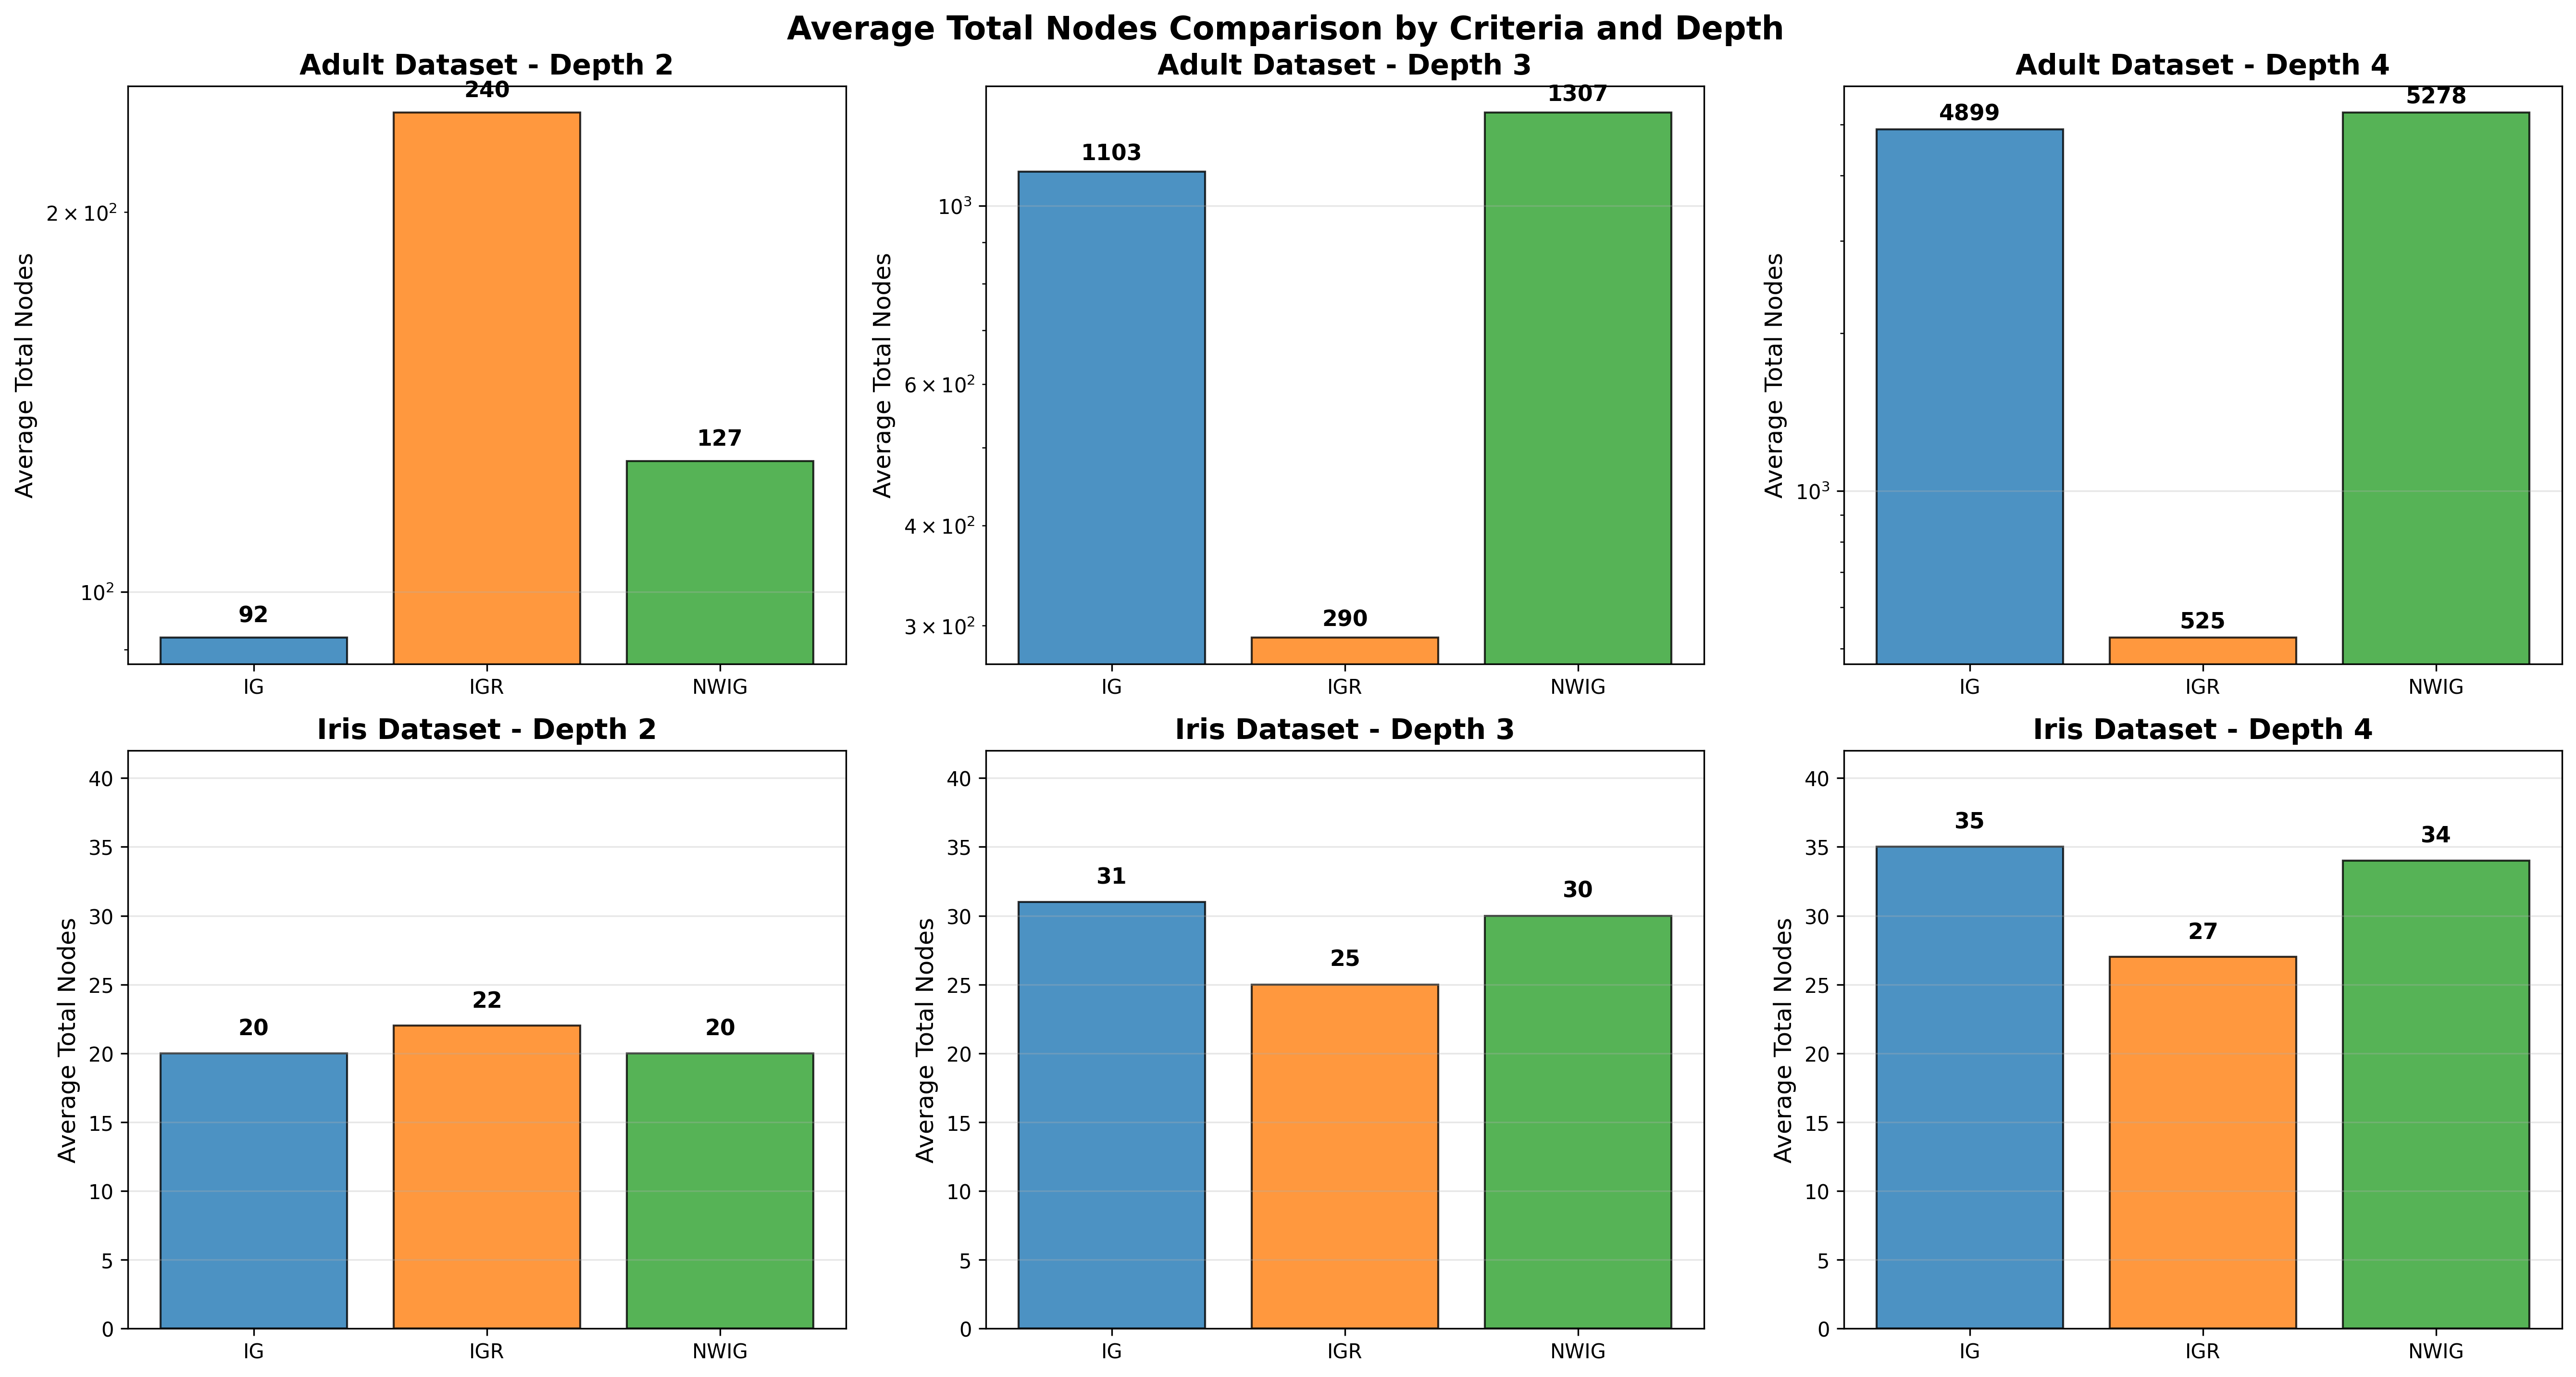
\includegraphics[width=0.95\textwidth]{nodes_bar_plots_by_depth.png}
\caption{Average Total Nodes by Criteria and Depth}
\label{fig:nodes_bars}
\end{figure}

Figure \ref{fig:nodes_combined} shows a direct comparison of node counts between datasets, highlighting the dramatic complexity differences.

\begin{figure}[H]
\centering
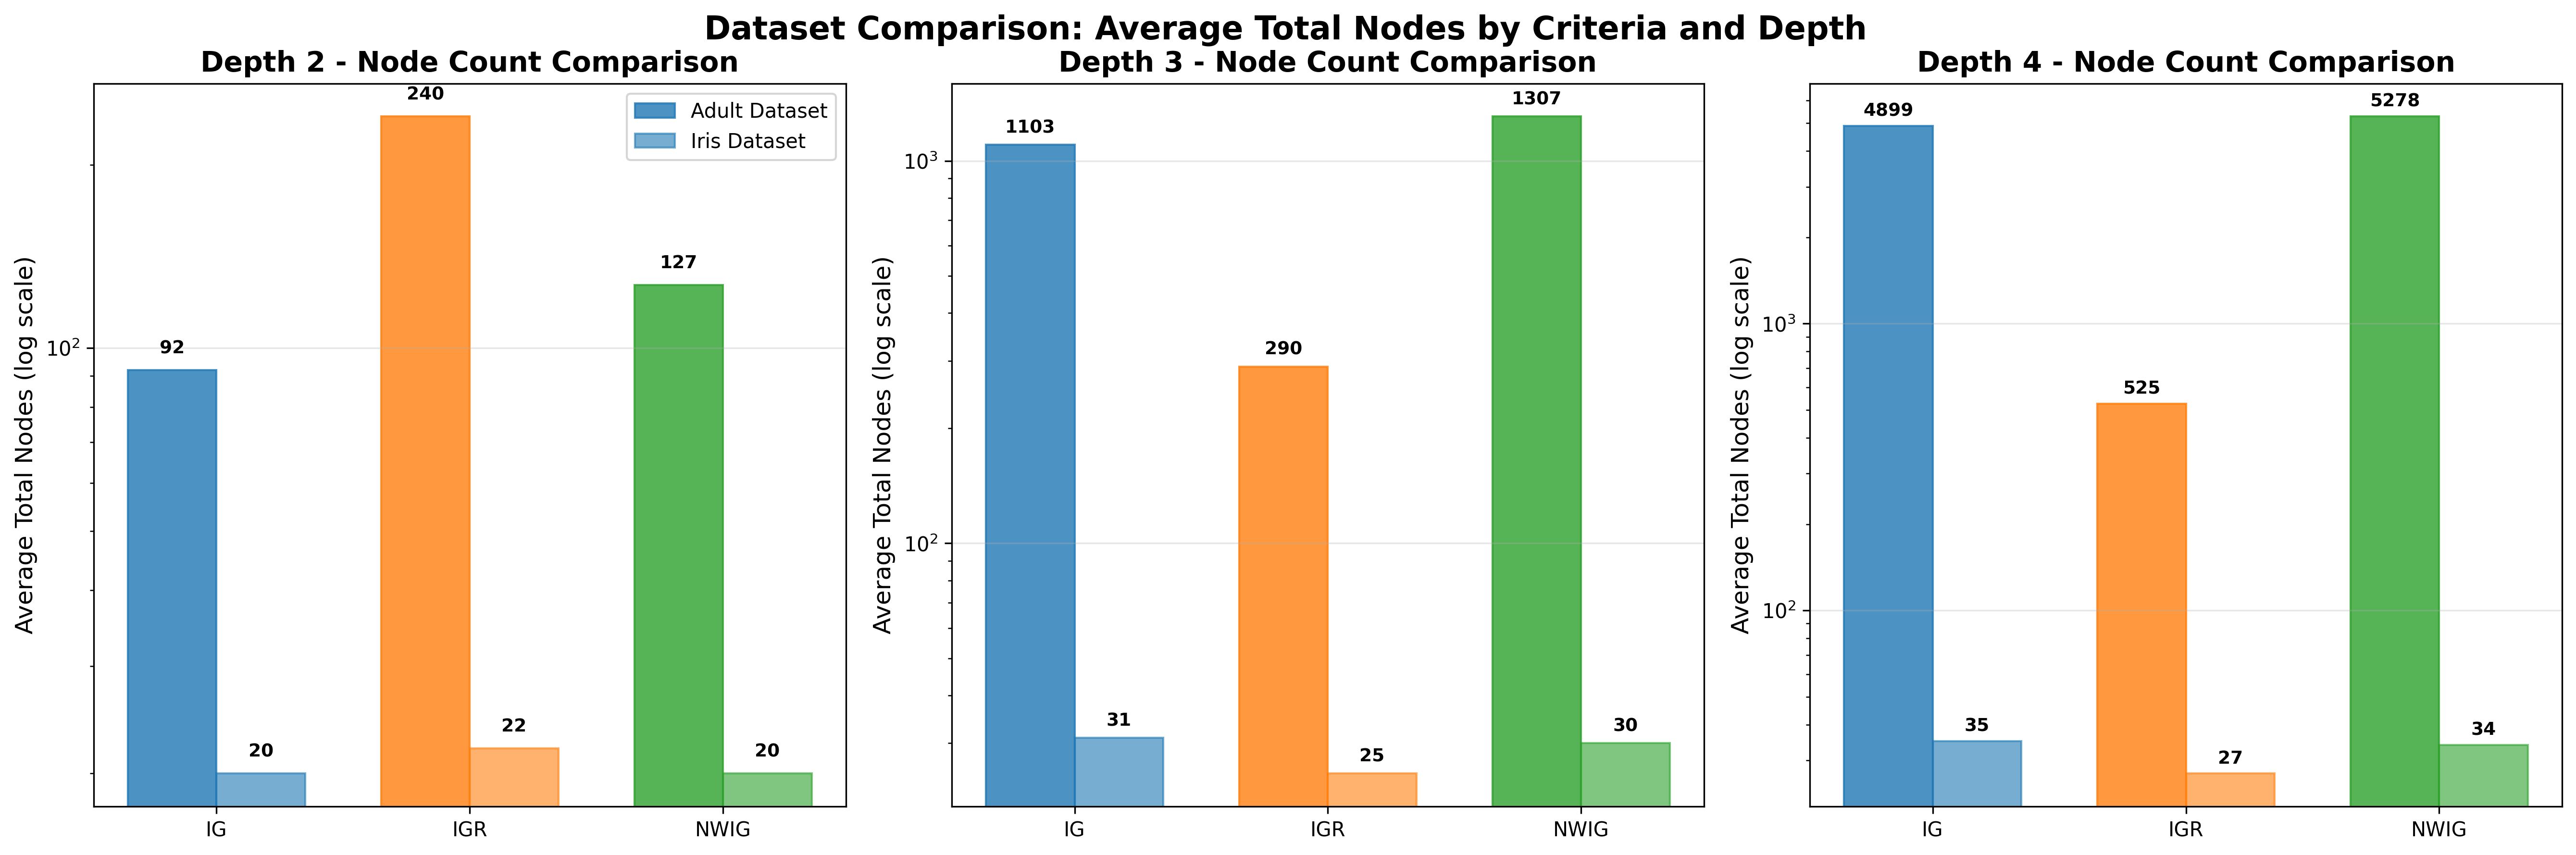
\includegraphics[width=0.95\textwidth]{combined_nodes_bar_comparison_by_depth.png}
\caption{Node Count Comparison Between Datasets}
\label{fig:nodes_combined}
\end{figure}

\section{Observations and Analysis}

\subsection{Key Findings}

\subsubsection{Information Gain Ratio (IGR) Superiority}
\begin{itemize}
    \item \textbf{Consistent Best Performance}: IGR achieved the highest accuracy across most depth-dataset combinations
    \item \textbf{Adult Dataset}: IGR peaked at 86.02\% (depth 4), significantly outperforming IG (82.05\%) and NWIG (81.76\%)
    \item \textbf{Iris Dataset}: IGR achieved 95.00\% accuracy at depth 3, the highest among all configurations
\end{itemize}

\subsubsection{Overfitting Resistance}
\begin{itemize}
    \item \textbf{IG and NWIG Overfitting}: Both criteria showed performance degradation at depth 4 for the Adult dataset
    \item \textbf{IGR Robustness}: IGR continued improving with increased depth, suggesting better resistance to overfitting
    \item \textbf{Tree Complexity}: IGR produced significantly smaller trees (525 nodes vs. 4,899 for IG and 5,278 for NWIG at depth 4)
\end{itemize}

\subsubsection{Computational Efficiency Trade-offs}
\begin{itemize}
    \item \textbf{Training Time}: IGR required moderate training time, avoiding the exponential growth seen in IG and NWIG
    \item \textbf{Testing Efficiency}: Despite larger initial testing times at shallow depths, IGR maintained efficient testing at depth 4
    \item \textbf{Scalability}: IGR's controlled node growth suggests better scalability for larger datasets
\end{itemize}

\subsection{Dataset-Specific Patterns}

\subsubsection{Adult Dataset (Large, Complex)}
\begin{itemize}
    \item \textbf{Depth Sensitivity}: Significant performance variations with depth changes
    \item \textbf{Criterion Impact}: Choice of splitting criterion critically affects both accuracy and computational cost
    \item \textbf{Overfitting Evidence}: Clear overfitting patterns in IG and NWIG at maximum depth
\end{itemize}

\subsubsection{Iris Dataset (Small, Simple)}
\begin{itemize}
    \item \textbf{High Baseline Performance}: All criteria achieved $\geq90$\% accuracy
    \item \textbf{Limited Depth Benefit}: Minimal improvement beyond depth 3
    \item \textbf{Criterion Robustness}: Less dramatic differences between criteria, though IGR still superior
\end{itemize}

\section{Conclusions}

\subsection{Primary Recommendations}
\begin{enumerate}
    \item \textbf{Prefer IGR for Decision Tree Construction}: Consistently superior performance across datasets and depths
    \item \textbf{Optimal Depth Selection}: Depth 3-4 provides best accuracy-complexity balance for most scenarios
    \item \textbf{Dataset Considerations}: Simple datasets (like Iris) may not require deep trees, while complex datasets benefit from careful depth tuning
\end{enumerate}

\subsection{Theoretical Implications}
\begin{itemize}
    \item \textbf{Bias Reduction}: IGR's normalization effectively reduces bias toward multi-valued attributes
    \item \textbf{Overfitting Prevention}: The gain ratio mechanism provides implicit regularization
    \item \textbf{Scalability : IGR's efficiency makes it suitable for larger, real-world applications}
\end{itemize}

\end{document}
